\documentclass{scrartcl}
\usepackage{xcolor, tikz}
\usepackage{pgfplots}
\pgfplotsset{compat=newest}
\pagestyle{empty}
\definecolor{pdg2112}{RGB}{228,26,28}
\definecolor{pdg2212}{RGB}{55,126,184}
\definecolor{pdg1000010020}{RGB}{153,153,153}
\definecolor{pdg1000020040}{RGB}{166,86,40}
\definecolor{pdg11}{RGB}{152,78,163}
\definecolor{pdg1000010030}{RGB}{153,153,153}
\definecolor{pdg22}{RGB}{77,175,74}
\definecolor{pdg1000060120}{RGB}{153,153,153}
\begin{document}
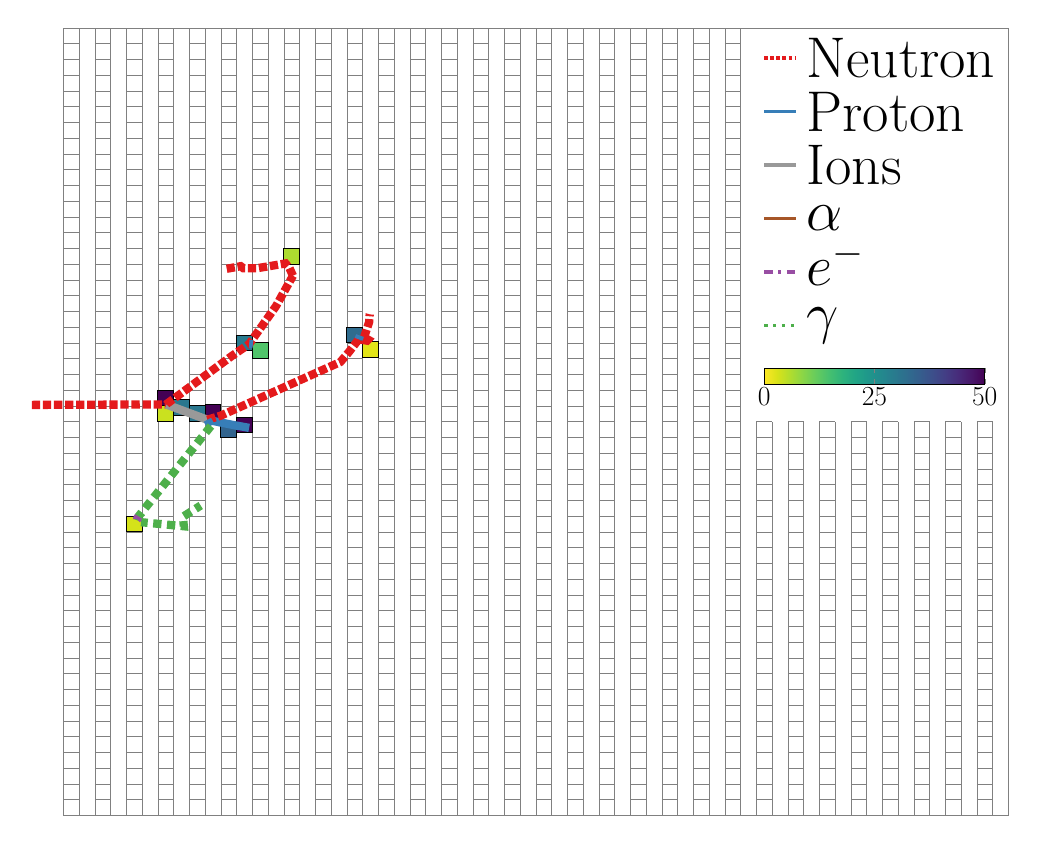
\begin{tikzpicture}[scale=0.4]
\draw[step=0.5,very thin,gray] (21.999000,-12.499) grid (22.500000,0);
\draw[step=0.5,very thin,gray] (22.999000,-12.499) grid (23.500000,0);
\draw[step=0.5,very thin,gray] (23.999000,-12.499) grid (24.500000,0);
\draw[step=0.5,very thin,gray] (24.999000,-12.499) grid (25.500000,0);
\draw[step=0.5,very thin,gray] (25.999000,-12.499) grid (26.500000,0);
\draw[step=0.5,very thin,gray] (26.999000,-12.499) grid (27.500000,0);
\draw[step=0.5,very thin,gray] (27.999000,-12.499) grid (28.500000,0);
\draw[step=0.5,very thin,gray] (28.999000,-12.499) grid (29.500000,0);
\draw[step=0.5,very thin,gray] (-0.001000,-12.499) grid (0.500000,12.499);
\draw[step=0.5,very thin,gray] (0.999000,-12.499) grid (1.500000,12.499);
\draw[step=0.5,very thin,gray] (1.999000,-12.499) grid (2.500000,12.499);
\draw[step=0.5,very thin,gray] (2.999000,-12.499) grid (3.500000,12.499);
\draw[step=0.5,very thin,gray] (3.999000,-12.499) grid (4.500000,12.499);
\draw[step=0.5,very thin,gray] (4.999000,-12.499) grid (5.500000,12.499);
\draw[step=0.5,very thin,gray] (5.999000,-12.499) grid (6.500000,12.499);
\draw[step=0.5,very thin,gray] (6.999000,-12.499) grid (7.500000,12.499);
\draw[step=0.5,very thin,gray] (7.999000,-12.499) grid (8.500000,12.499);
\draw[step=0.5,very thin,gray] (8.999000,-12.499) grid (9.500000,12.499);
\draw[step=0.5,very thin,gray] (9.999000,-12.499) grid (10.500000,12.499);
\draw[step=0.5,very thin,gray] (10.999000,-12.499) grid (11.500000,12.499);
\draw[step=0.5,very thin,gray] (11.999000,-12.499) grid (12.500000,12.499);
\draw[step=0.5,very thin,gray] (12.999000,-12.499) grid (13.500000,12.499);
\draw[step=0.5,very thin,gray] (13.999000,-12.499) grid (14.500000,12.499);
\draw[step=0.5,very thin,gray] (14.999000,-12.499) grid (15.500000,12.499);
\draw[step=0.5,very thin,gray] (15.999000,-12.499) grid (16.500000,12.499);
\draw[step=0.5,very thin,gray] (16.999000,-12.499) grid (17.500000,12.499);
\draw[step=0.5,very thin,gray] (17.999000,-12.499) grid (18.500000,12.499);
\draw[step=0.5,very thin,gray] (18.999000,-12.499) grid (19.500000,12.499);
\draw[step=0.5,very thin,gray] (19.999000,-12.499) grid (20.500000,12.499);
\draw[step=0.5,very thin,gray] (20.999000,-12.499) grid (21.500000,12.499);
\draw[very thin,gray] (0,-12.5) -- (30,-12.5) -- (30,12.5) -- (0,12.5);
\definecolor{tempcolor}{rgb}{0.835270,0.886029,0.102646}\draw[fill=tempcolor,fill opacity=1] (2.000000,-3.500000) rectangle (2.500000,-3.000000);
\definecolor{tempcolor}{rgb}{0.793760,0.880678,0.120005}\draw[fill=tempcolor,fill opacity=1] (3.000000,0.000000) rectangle (3.500000,0.500000);
\definecolor{tempcolor}{rgb}{0.267004,0.004874,0.329415}\draw[fill=tempcolor,fill opacity=1] (3.000000,0.500000) rectangle (3.500000,1.000000);
\definecolor{tempcolor}{rgb}{0.165117,0.467423,0.558141}\draw[fill=tempcolor,fill opacity=1] (3.500000,0.207050) rectangle (4.000000,0.707050);
\definecolor{tempcolor}{rgb}{0.165117,0.467423,0.558141}\draw[fill=tempcolor,fill opacity=1] (4.000000,0.000000) rectangle (4.500000,0.500000);
\definecolor{tempcolor}{rgb}{0.267004,0.004874,0.329415}\draw[fill=tempcolor,fill opacity=1] (4.500000,0.033703) rectangle (5.000000,0.533703);
\definecolor{tempcolor}{rgb}{0.197636,0.391528,0.554969}\draw[fill=tempcolor,fill opacity=1] (5.000000,-0.500000) rectangle (5.500000,0.000000);
\definecolor{tempcolor}{rgb}{0.267004,0.004874,0.329415}\draw[fill=tempcolor,fill opacity=1] (5.500000,-0.356239) rectangle (6.000000,0.143761);
\definecolor{tempcolor}{rgb}{0.160665,0.478540,0.558115}\draw[fill=tempcolor,fill opacity=1] (5.500000,2.247629) rectangle (6.000000,2.747629);
\definecolor{tempcolor}{rgb}{0.311925,0.767822,0.415586}\draw[fill=tempcolor,fill opacity=1] (6.000000,2.000000) rectangle (6.500000,2.500000);
\definecolor{tempcolor}{rgb}{0.678489,0.863742,0.189503}\draw[fill=tempcolor,fill opacity=1] (7.000000,5.000000) rectangle (7.500000,5.500000);
\definecolor{tempcolor}{rgb}{0.183898,0.422383,0.556944}\draw[fill=tempcolor,fill opacity=1] (9.000000,2.500000) rectangle (9.500000,3.000000);
\definecolor{tempcolor}{rgb}{0.886271,0.892374,0.095374}\draw[fill=tempcolor,fill opacity=1] (9.500000,2.049908) rectangle (10.000000,2.549908);
\draw[color=pdg2112, line width=3pt, densely dotted] (-1.0029926656072803, 0.5315310134710203) -- (-0.003012750611355841, 0.5350983357090808) -- (0.48999999999998634, 0.5368571063829002) -- (0.9899999999999863, 0.5386408033274908) -- (1.4899999999999864, 0.5404245002720814) -- (1.9899999999999864, 0.5422081972166721) -- (2.4683741583881327, 0.5439147462660483) -- (2.4899999999999864, 0.5438878943517402) -- (2.9899999999999864, 0.5432670650034558) -- (3.270547079417702, 0.5429187212824997);
\draw[color=pdg1000010030, line width=3pt, solid] (3.270547079417702, 0.5429187212824997);
\draw[color=pdg1000020040, line width=3pt, solid] (3.270547079417702, 0.5429187212824997);
\draw[color=pdg1000010020, line width=3pt, solid] (3.270547079417702, 0.5429187212824997);
\draw[color=pdg2212, line width=3pt, solid] (3.270547079417702, 0.5429187212824997) -- (3.3092168717977986, 0.5581246956579015) -- (3.3268458114555415, 0.5647070792488392) -- (3.3462696007189607, 0.5691561100452529) -- (3.3611177122380242, 0.5729355480972146) -- (3.373021002502719, 0.576594271059447) -- (3.3823796829798995, 0.5797168677686122) -- (3.3896732478131297, 0.5821526538160928) -- (3.395161625781043, 0.5842316880692632);
\draw[color=pdg1000010020, line width=3pt, solid] (3.270547079417702, 0.5429187212824997) -- (3.360114537165532, 0.51) -- (3.379023477266037, 0.503) -- (3.3952032411397797, 0.497) -- (3.4086863777012466, 0.492) -- (3.490000000000009, 0.461913140633346) -- (3.990000000000009, 0.2772930428136021) -- (4.489999999999986, 0.08948922162782424) -- (4.572100562891774, 0.060318645183074726);
\draw[color=pdg2212, line width=3pt, solid] (4.572100562891774, 0.060318645183074726) -- (4.843630325652839, 0.0028136905912220025) -- (4.990000000000009, -0.02657537278186743) -- (5.196086087491108, -0.06697793331579367) -- (5.343464276008899, -0.09693473793855958) -- (5.461417815882283, -0.11931160562184735) -- (5.489999999999986, -0.12441803815923955) -- (5.595453772388851, -0.14329521794365524) -- (5.664636080291325, -0.15554065206350237) -- (5.719875521180711, -0.16531356399795716) -- (5.764534092549297, -0.17317018378802523) -- (5.800075240787601, -0.17985306708284243) -- (5.828852937053216, -0.18506530741241758) -- (5.851836079633972, -0.18954181545723411) -- (5.870462845818975, -0.19299081943874724) -- (5.885416419665921, -0.19568291889973802) -- (5.8971987095636225, -0.1978584813505936);
\draw[color=pdg2112, line width=3pt, densely dotted] (4.572100562891774, 0.060318645183074726) -- (4.989999999999986, 0.1881426479681991) -- (5.490000000000009, 0.4116297844200454) -- (5.681813672606381, 0.4976930050794156) -- (5.698375366729602, 0.5051239286233496) -- (5.990000000000009, 0.6359704674639985) -- (6.490000000000009, 0.8603111505079586) -- (6.955790143622858, 1.0693025084589562) -- (6.972351837746101, 1.07673343200289) -- (6.990000000000009, 1.0846518335519113) -- (7.490000000000009, 1.3089925165958713) -- (7.5927783791311185, 1.3551072601487266) -- (7.609340073254339, 1.3625381836926607) -- (7.990000000000009, 1.533333199639829) -- (8.490000000000009, 1.7576738826837892) -- (8.793456066420594, 1.8938289651130495) -- (8.972793593028655, 2.1033898500369568) -- (8.99461254340631, 2.12888590005914) -- (9.002999999999997, 2.138686876236733) -- (9.060932772466549, 2.206382931233171) -- (9.279917578793539, 2.49) -- (9.376855069204657, 2.61554810237818) -- (9.490000000000009, 2.5967984542965694) -- (9.543007423979066, 2.5880144059230936) -- (9.55842870666147, 2.5854588904330935) -- (9.57164694896071, 2.583268448584522) -- (9.582662150876718, 2.581443080377379) -- (9.641923577168473, 2.57162265908255) -- (9.67173494804174, 2.6026643394405413) -- (9.598558352830263, 2.6436434388004866) -- (9.550265816350224, 2.687672104575059) -- (9.573656808332203, 2.7585461302585514) -- (9.577663102576206, 2.7706850853470595) -- (9.581097069071053, 2.7810899039943515) -- (9.583958707816759, 2.7897605862004276) -- (9.706649619305812, 3.16151048114756) -- (9.724590101806825, 3.4053942218126556) -- (9.725145344514772, 3.4072963555847293);
\draw[color=pdg2212, line width=3pt, solid] (9.724590101806825, 3.4053942218126556);
\draw[color=pdg1000060120, line width=3pt, solid] (9.67173494804174, 2.6026643394405413);
\draw[color=pdg2212, line width=3pt, solid] (9.641923577168473, 2.57162265908255);
\draw[color=pdg2212, line width=3pt, solid] (9.376855069204657, 2.61554810237818) -- (9.387237029336394, 2.647064089298129) -- (9.396223116674856, 2.6724348340766375) -- (9.403388912632385, 2.693035921669356) -- (9.409132784321901, 2.7093263935754046) -- (9.413825694830303, 2.722450139084037) -- (9.41761177154749, 2.7329747069387773);
\draw[color=pdg1000060120, line width=3pt, solid] (8.793456066420594, 1.8938289651130495);
\draw[color=pdg2212, line width=3pt, solid] (4.572100562891774, 0.060318645183074726) -- (4.597515355273413, 0.01389427897022327) -- (4.617508848289003, -0.022682304363903866) -- (4.633953578683145, -0.05166437929627462) -- (4.647386352917328, -0.07487400971997764) -- (4.65809020271854, -0.09351100505278492) -- (4.666755651272115, -0.10872944153543566) -- (4.67374026367479, -0.12119300419763912) -- (4.679391441573398, -0.13126325204285197);
\draw[color=pdg1000060120, line width=3pt, solid] (4.684170688073573, -0.13951760625725443);
\draw[color=pdg22, line width=3pt, dotted] (4.684170688073573, -0.13951760625725443) -- (4.510000000000014, -0.35663758298332704) -- (4.403018485515713, -0.49000000000000005) -- (4.009999999999991, -0.97993412939864) -- (3.509999999999991, -1.6032306758139303) -- (3.199738916082174, -1.9900000000000002) -- (3.009999999999991, -2.2265272222292074) -- (2.509999999999991, -2.8498237686444976) -- (2.397552536459807, -2.9899999999999993) -- (2.3886002800712958, -3.0099999999999993) -- (2.4623739042263653, -3.0397436377515783) -- (2.4899999999999864, -3.0832255077529984) -- (2.492000000000007, -3.086373391576905) -- (2.4970000000000026, -3.0942431011366027) -- (2.5029999999999974, -3.103686752608248) -- (2.507999999999993, -3.111556462167961) -- (2.5100000000000136, -3.114704345991858) -- (2.546585547712857, -3.172287872908439) -- (2.523831799512686, -3.196189058078802) -- (2.5100000000000136, -3.1953095002215135) -- (2.507999999999993, -3.195182321128658) -- (2.506119590855428, -3.195062746764056) -- (2.5029999999999974, -3.1948643733965203) -- (2.4970000000000256, -3.1944828361179556) -- (2.492000000000007, -3.1941648883858162) -- (2.4899999999999864, -3.194037709292961) -- (2.4643974872164565, -3.1924096571176506) -- (2.4899999999999864, -3.1948373365789733) -- (2.7798715604887776, -3.2223235149775418) -- (2.9899999999999864, -3.2422482974062823) -- (3.4899999999999864, -3.289659258233589) -- (3.823426233770101, -3.3212753744497334) -- (3.7944479433183913, -3.0198473027626855) -- (3.8219116931313692, -3.0024921459196148) -- (3.990000000000009, -2.8962721668906184) -- (4.358608149413453, -2.663337760982144);
\draw[color=pdg11, line width=3pt, dashdotted] (4.358608149413453, -2.663337760982144);
\draw[color=pdg11, line width=3pt, dashdotted] (3.7944479433183913, -3.0198473027626855);
\draw[color=pdg11, line width=3pt, dashdotted] (3.823426233770101, -3.3212753744497334);
\draw[color=pdg11, line width=3pt, dashdotted] (2.4643974872164565, -3.1924096571176506);
\draw[color=pdg11, line width=3pt, dashdotted] (2.523831799512686, -3.196189058078802);
\draw[color=pdg11, line width=3pt, dashdotted] (2.546585547712857, -3.172287872908439);
\draw[color=pdg11, line width=3pt, dashdotted] (2.4623739042263653, -3.0397436377515783);
\draw[color=pdg11, line width=3pt, dashdotted] (2.3832418407884233, -3.007839614377516) -- (2.3571256219955785, -3.0492043839889034) -- (2.344121978248313, -3.0782514926035045) -- (2.3447350385324626, -3.091227783331449) -- (2.337938026313691, -3.0973109661761606);
\draw[color=pdg2212, line width=3pt, solid] (4.684170688073573, -0.13951760625725443);
\draw[color=pdg2112, line width=3pt, densely dotted] (3.270547079417702, 0.5429187212824997) -- (3.297779483432032, 0.5752967599803902) -- (3.490000000000009, 0.7169364508665459) -- (3.918501171373464, 1.0326820046780592) -- (3.990000000000009, 1.0853666616865794) -- (4.490000000000009, 1.4537968725066277) -- (4.837672706630269, 1.7099831297069499) -- (4.990000000000009, 1.8222270833266652) -- (5.217686155676438, 1.9899999999999998) -- (5.2271859195318715, 1.9969999999999999) -- (5.2353285742650995, 2.0029999999999997) -- (5.242114119876123, 2.008) -- (5.345703738832026, 2.0843310903013785) -- (5.489999999999986, 2.1834889876860175) -- (5.830087939277791, 2.417191543190244) -- (5.896872983325375, 2.463085071483318) -- (5.989999999999986, 2.5945484371126435) -- (6.0029999999999974, 2.612899972619823) -- (6.2701329793644165, 2.99) -- (6.490000000000009, 3.3003767258500014) -- (6.5029999999999974, 3.318728261357149) -- (6.746415779218137, 3.6623477471515478) -- (6.990000000000009, 4.098034073819997) -- (6.99699999999998, 4.110554606869628) -- (7.0029999999999974, 4.121286492340807) -- (7.007999999999993, 4.130229730233429) -- (7.209140948102936, 4.49) -- (7.28846031004125, 4.631874384661162);
\draw[color=pdg1000020040, line width=3pt, solid] (7.28846031004125, 4.631874384661162);
\draw[color=pdg1000020040, line width=3pt, solid] (7.28846031004125, 4.631874384661162);
\draw[color=pdg1000020040, line width=3pt, solid] (7.28846031004125, 4.631874384661162);
\draw[color=pdg2112, line width=3pt, densely dotted] (7.28846031004125, 4.631874384661162) -- (7.17523126355186, 4.880467322158351) -- (7.080897496465832, 4.99) -- (7.0534151757283325, 5.021910229779502) -- (7.010000000000014, 5.014664801915422) -- (6.590157439970744, 4.944598542089662) -- (6.510000000000014, 4.931221308453404) -- (6.14837357844151, 4.870870564567381) -- (6.009999999999991, 4.87162199878538) -- (5.710952276670378, 4.873245969883439) -- (5.629129617523335, 4.9356034500859405) -- (5.509999999999991, 4.9135312430218745) -- (5.1853734535236295, 4.8533847865714845);
\draw[color=pdg2212, line width=3pt, solid] (5.1853734535236295, 4.8533847865714845);
\draw[color=pdg2212, line width=3pt, solid] (5.629129617523335, 4.9356034500859405);
\draw[color=pdg2212, line width=3pt, solid] (5.710952276670378, 4.873245969883439);
\draw[color=pdg2212, line width=3pt, solid] (6.14837357844151, 4.870870564567381);
\draw[color=pdg2212, line width=3pt, solid] (7.0534151757283325, 5.021910229779502);
\draw[color=pdg2212, line width=3pt, solid] (5.896872983325375, 2.463085071483318) -- (5.924601501870984, 2.461301688441498) -- (5.947086420597361, 2.4600191073804694) -- (5.964585291348749, 2.4592500728922038) -- (5.9781511849587785, 2.4594236601610904) -- (5.989052107717521, 2.458728667311945) -- (5.9970000000000026, 2.4582404053071523) -- (6.0029999999999974, 2.4575915811843636) -- (6.008000000000015, 2.4570508944153726) -- (6.015058424726362, 2.456260516845886);
\draw[color=pdg2112, very thick, densely dotted] (22.25,11.550000) -- (23.25,11.550000) node [right,black] {\huge{Neutron}};
\draw[color=pdg2212, very thick, solid] (22.25,9.850000) -- (23.25,9.850000) node [right,black] {\huge{Proton}};
\draw[color=pdg1000010020, very thick, solid] (22.25,8.150000) -- (23.25,8.150000) node [right,black] {\huge{Ions}};
\draw[color=pdg1000020040, very thick, solid] (22.25,6.450000) -- (23.25,6.450000) node [right,black] {\huge{$\alpha$}};
\draw[color=pdg11, very thick, dashdotted] (22.25,4.750000) -- (23.25,4.750000) node [right,black] {\huge{$e^-_{\vphantom{-}}$}};
\draw[color=pdg22, very thick, dotted] (22.25,3.050000) -- (23.25,3.050000) node [right,black] {\huge{$\gamma$}};
\begin{axis}[%
    at={(22.25cm,2cm)}, %4.75
    hide axis,
    scale only axis,
    height=0pt,
    width=0pt,
    colormap={reverse viridis}{
       indices of colormap={
       \pgfplotscolormaplastindexof{viridis},...,0 of viridis}
    },
    colorbar horizontal,
    point meta min=0,
    point meta max=50,
    label style={font=\Huge},
    tick label style={font=\Huge},
    colorbar style={
       width=7cm,
       xtick={50, 25, 0},
    }]
\end{axis}
\end{tikzpicture}
\end{document}
